\documentclass[a4paper]{book}
\newcommand\hmmax{0}
\newcommand\bmmax{0}
\usepackage{booktabs}
\usepackage{mparhack}

%% Language and font encodings
\usepackage[english]{babel}
\usepackage[utf8x]{inputenc}
\usepackage[T1]{fontenc}
\usepackage{gensymb}
\usepackage{pdfpages}
\usepackage[algoruled]{algorithm2e}

\usepackage{chngcntr}

\counterwithin*{equation}{section}

\usepackage[bitstream-charter]{mathdesign}
\let\circledS\undefined
%% Sets page size and margins
\usepackage[a4paper,top=2cm,bottom=4cm,left=1cm,right=6cm,marginparwidth=4cm, marginparsep=1cm]{geometry}

%% Useful packages
\usepackage{amsmath}
\usepackage{bm}
\usepackage[makeroom]{cancel}
\usepackage{enumitem}
\usepackage{listings}
\usepackage{multirow}
\usepackage{amssymb}
\usepackage{float}
\usepackage{graphicx}
\usepackage[colorinlistoftodos]{todonotes}
\usepackage[colorlinks=true, allcolors=blue]{hyperref}
\usepackage[final]{matlab-prettifier}
\usepackage{courier}
\usepackage{algorithm}
\usepackage[noend]{algpseudocode}
\usepackage[]{appendix}
\usepackage{wrapfig}
\usepackage[final]{matlab-prettifier}

\renewcommand\labelitemi{$\bullet$}

\definecolor{codecol}{rgb}{0.94, 0.94, 0.94}
\definecolor{dgreen}{rgb}{0.1, 0.49, 0.1}

\newcommand{\ea}{\nonumber \\}
\lstset{basicstyle=\footnotesize\ttfamily,breaklines=true}
\lstset{framextopmargin=50pt,frame=bottomline}

\newcommand{\norm}[2]{\left\Vert#1\right\Vert_{#2}}
\newcommand{\question}[1]{{\color{red}\textbf{Question: }\emph{#1}}}
\newcommand{\action}[1]{{\color{blue}\textbf{Action: }\emph{#1}}}
\newcommand{\epdp}{$(\epsilon, \delta)$-DP}
\newcommand{\alg}{$\mathcal{A}$}
\newcommand{\data}{$\mathcal{D}$}
\newcommand{\vect}[1]{\boldsymbol{\mathbf{#1}}}
\newcommand{\normaldist}[2]{$\mathcal{N}(#1, #2)$}
\newcommand{\expt}[2]{\mathbb{E}_{#2}[#1]}
\newcommand{\prob}[2]{\mathbb{P}_{#2}[#1]}
\newcommand{\model}[1]{\mathcal{M}_{#1}}
\newcommand{\indep}{\raisebox{0.05em}{\rotatebox[origin=c]{90}{$\models$}}}
\newcommand{\mset}[3]{\lbrace {#1}_{#2} \rbrace_{#2=1}^{#3} }

\newcommand{\ix}[1]{%
  \leavevmode % if at the start of a paragraph
  \marginpar{\small\emph{#1}}% the note
}

\newcommand{\qx}[1]{%
	\leavevmode % if at the start of a paragraph
	\marginpar{\color{blue}\small\emph{#1}}% the note
}
\newcommand{\marfig}[2]{
  \marginpar{ \includegraphics[width=\marginparwidth]{#1} \centering \text{\small #2} }
}

\DeclareMathAlphabet{\altmathcal}{OMS}{cmsy}{m}{n}

\title{\textbf{4F7 Statistical Signal Analysis}\\
\textit{Course Notes}
}
\author{Mrinank Sharma}

\begin{document}
%\maketitle
% \tableofcontents
\chapter{4F7 Statistical Signal Analysis}
Please note that the margins of these notes can be used to check factual recall simply by covering up the right hand text.

\section{State Space Models}
\subsection{Preliminaries}
\ix{White Noise Sequences}The notation $ W_n \sim \text{WN}(0, Q_n)$ denotes a sequence of random vectors, $W_1, W_2, \ldots$ with zero mean and second moment
\begin{align}
\expt{W_n W_m^{T}}{} = \begin{cases}
0 \hspace{1cm} &m\neq n \\
Q_n & m=n
\end{cases}
\end{align}
\ix{State Space Model} A state space model for a time series, $\lbrace Y_n \rbrace$ consists of two equations:
\begin{align}
Y_n &= G_n X_n + V_n  &&n = 1, 2, \ldots &&&\text{(observation)}\\
X_{n+1} &= F_n X_n + W_{n}  &&n = 1, 2, \ldots &&&\text{(evolution)}
\end{align}
where $V_n \sim \text{WN}(0, R_n)$ and $\lbrace G_n \rbrace$ is some \emph{deterministic} sequence of matrices. Similarly, $W_n \sim \text{WN}(0, Q_n)$ and $\lbrace F_n \rbrace$ is some deterministic sequence of matrices. In certain models, observations may be noiseless. 

\ix{Additional assumptions}Additionally, the following assumptions are made:
\begin{align}
\text{cov}[X_1, W_n] &= 0 \hspace{0.25cm} n \geq 1 \\
\text{cov}[X_1, V_n] &= 0 \hspace{0.25cm} n \geq 1 \\ 
\text{cov}[V_n, W_n] &= 0 \hspace{0.25cm} n \geq 1,\  m \geq 1 
\end{align}
Note that these assumptions are made on \textbf{correlation, not independence}. Note that $\text{cov}(X, Y) = \expt{XY^{T}}{} - \expt{X}{}\expt{Y}{}^{T}$. For example, $X \sim \altmathcal{N}(0, 1)$ and $Y = |X|$ are not independent, but they are uncorrelated. 

It is possible to express $X_n$ as a linear function of $X_1$ and $\lbrace W_i \rbrace_{i=1}^{n-1}$:
\begin{align}
X_n = \Big(\prod_{i=1}^{n-1} F_i \Big)X_1 + \sum_{i=1}^{n-1} W_i \prod_{j=i}^{n-1} F_i 
\end{align}
The state at time $n$ is a linear function of the initial state and driving noise sequence. Using this form of $X_n$, it is possible to prove the following facts: \qx{Try proving these yourself!}
\begin{align}
\expt{X_m W_n^{T}}{} &= 0 \hspace{1cm} m \leq n \\
\expt{Y_m W_n^{T}}{} &= 0 \hspace{1cm} m \leq n \\
\expt{X_m V_n^{T}}{} &= 0 \hspace{1cm} \forall m, n \\
\expt{Y_m V_n^{T}}{} &= 0 \hspace{1cm} m < n
\end{align}
In situations where there is no mention of a hidden state process, if a time series $Y_n$ can be expressed through some hidden state process, then this time series has a state-space representation.

\subsection{Linear Prediction}
\textbf{Note: } for this section, a scalar valued state-space model is used. 

\ix{Linear Prediction} Given random variables $Y_1, \ldots, Y_n$ and some random variable $X$ which we seek to estimate, linear predictors of X using $Y_1, \ldots, Y_n$ take the form:
\begin{align}
\hat{X} = h_0 + \sum_{i=1} h_i Y_i
\end{align}
for some constants $h_0, \ldots, h_n$. The best linear predictor is the predictor with coefficients $h_0^*, \ldots, h_n^*$ which satisfy:
\begin{align}
h_0^*, \ldots, h_n^* = \text{arg} \min_{(h_0, \ldots, h_n)} \mathbb{E}\ \Big[ \Big( h_0 + \sum_{i=1} h_i Y_i - X\Big)^2 \Big]
\end{align}
The best linear predictor (i.e. the predictor with the above coefficients) is denoted as $K[\cdot| \cdot]$ i.e. a function of two arguments. 

By\qx{Try proving this yourself!} differentiating the cost function with respect to the filter parameter, it is possible to show that:
\begin{align}
h_0 &= \expt{X}{} - \sum_i h_i  \expt{Y_i}{} \\
0 &= \expt{ \Big\lbrace \Big(\sum_i h_i (Y_i - \expt{Y_i}{})\Big) - (X - \expt{X}{}) \Big\rbrace (Y_k - \expt{Y_k}{})}{} \hspace{0.25cm} \forall k \label{eq:kalman_cov}
\end{align}
Note that in the proof, the additional term of $\expt{Y_i}{}$ can be added as the expectation of terms corresponding to this term are zero. Writing $\vect{p} = \begin{bmatrix}
\text{cov}[X, Y_i] & \cdots & \text{cov}[X, Y_n]
\end{bmatrix}^{T}$, Eq. \ref{eq:kalman_cov} can be written as:
\begin{align}
\bm{\Sigma}_Y \vect{h} = \vect{p}. 
\end{align}
Therefore, \ix{The Kalman Filter}the best linear predictor is of the form:
\begin{align}
K[X|Y_1, \ldots, Y_n] = \expt{X}{} + \sum_{i=1}^{N} h_i (Y_i - \expt{Y_i}{})
\end{align}
\ix{Properties of the Kalman Filter}where $\bm{\Sigma}_Y \vect{h} = \vect{p}$. This has the following properties:
\begin{itemize}
	\item The error of the estimate has zero mean.
	\begin{align}
	\expt{X - K[X|Y_{1:n}]}{} = 0
	\end{align}
	
	\item The error is orthogonal to all $Y_i$.
	\begin{align}
	\expt{(X - K[X|Y_{1:n}])Y_i}{} = 0
	\end{align}
	This follows directly from Eq. \ref{eq:kalman_cov}, noting that the term corresponding to $\expt{Y_i}{}$ is zero. 
	
	\item If $\text{cov}[Y_i, Y_n] = 0$ for $i < n$, then: \qx{Prove this property, and the below properties. }
	\begin{align}
	K[X | Y_{1:n}] = K [X|Y_{1:n-1}] + K[X|Y_n] - \expt{X}{}
	\end{align}
	Note: proof hinges on the condition ensuring that the coefficients do not change. 
	
	\item Linearity:
	\begin{align}
	K[aX + bU + c | Y_{1:n}] = aK[X | Y_{1:n}] + bK[U | Y_{1:n}] + c
	\end{align}
	
	\item If $\tilde{\vect{Y}} = \vect{C} \vect{Y} + \vect{b}$ where $\tilde{C}$ is an invertible matrix, then:
	\begin{align}
	K[X | Y_{1:n}] = K[X | \tilde{Y}_{1:n}]
	\end{align}
	This can be shown by showing that the filter coefficients obtained are effectively the same in both cases. 
	
	\item If $\text{cov}[U, Y_i] = 0$, then: 
	\begin{align}
	K[U|Y_{1:n}] = \expt{U}{}
	\end{align}
	
	\item $K[Y_i | Y_{1:n}] = Y_i$. 
\end{itemize}

\subsection{Kalman Filtering}
\ix{Objective}The objective is to compute the filter, $K[X_n | Y_{1:n}]$, recursively in time for a state-space model:
\begin{align}
Y_n &= g_nX_n + V_n \\
X_{n+1} &= f_nX_n + W_n 
\end{align}
for $n= 1, 2, \ldots$ with $V_n \sim \text{WN}(0, r_n)$ and $W_n \sim \text{WN}(0, q_n)$. Additionally, \begin{align}
\nonumber \text{cov}(X_1, W_n)= \text{cov}(X_1, V_n) = \text{cov}(V_m, W_n) = 0
\end{align} 
for all $n\geq1$ and $m \geq 1$. To derive the filter, it is assumed that $K[X_n | Y_{1:n}]$ has already been calculated. 

For the prediction step,\ix{Prediction} we seek to calculate $K[X_{n+1} | Y_{1:n}]$. It is straightforward to show that:\qx{Complete Proof}
\begin{align}
K[X_{n+1} | Y_{1:n}] = f_n K[X_n | Y_{1:N}] \label{eq:kalman_pred_1}
\end{align}
Similarly, it is easy to show that:
\begin{align}
K[Y_{n+1} | Y_{1:N}] = g_{n+1} f_n K[X_n | Y_{1:N}]
\end{align}
The mean square error is also updated sequentially. Denote the mean square error as $\sigma_n = \expt{(X_n - K[X_n | Y_{1:n}])^2}{}$. Then\ix{Prediction MSE Update}
\begin{align}
\underbrace{\expt{(X_{n+1} - K[X_{n+1} | Y_{1:n}])^2}{}}_{\bar{\sigma}_{n+1}} &= \expt{(f_nX_n + W_n - f_n K[X_n| Y_{1:n}])^2}{} \nonumber \\
&= f_n^2 \expt{(X_n - K[X_n | Y_{1:n}])^2}{} + \expt{W_n^2}{} + 2 f_n \underbrace{\expt{(X_n - K[X_n | Y_{1:n}])W_n}{}}_{0} \nonumber \\
&= f_n^2 \sigma_n + q_n \label{eq:kalman_pred_2}
\end{align}
i.e. the mean square error is inflated by $q_n$ due to the additional noise and scaled by $f_n$. \ix{Why is the final term zero?}The final term is zero because $X_n - K[X_n | Y_{1:n}]$ is linear in $(X_1, W_1, \ldots W_{n-1}, V_1, \ldots, V_{n})$. The expected value of this term multiplied by $W_n$ is zero. Together, Equations \ref{eq:kalman_pred_1} and \ref{eq:kalman_pred_2} make up the Kalman prediction step for a state-space model. 

\ix{Derivation of the Kalman Update Step}The \emph{innovations} are defined as:
\begin{align}
I_{n+1} = Y_{n+1} - K[Y_{n+1}|Y_{1:n}] = Y_{n+1} - g_{n+1} f_n K[X_n | Y_{1:n}]
\end{align}
these can be thought of as the unpredictable part of $Y$. Note that $\text{cov}(I_{n+1}, Y_i) = 0, i < n+1$ as the error is orthogonal to the inputs. Additionally, note that $Y_{n+1} = I_{n+1} + K[Y_{n+1}| Y_{1:n}]$, meaning that there is an invertible matrix and bias, $\vect{C}$ and $\vect{b}$ such that:\qx{Find these matrices}
\begin{align}
\nonumber \begin{bmatrix}
Y_{1:n} & I_{n+1}
\end{bmatrix}^T = \vect{C} \nonumber \begin{bmatrix}
Y_{1:n} & Y_{n+1}
\end{bmatrix}^T + \vect{b}
\end{align}
Therefore, 
\begin{align}
K[\cdot| Y_{1, n+1}] = K[\cdot | Y_{1:n}, I_{n+1}] = K[\cdot| Y_{1:n}] + K[\cdot| I_{n+1}] - \expt{\cdot}{}
\end{align}
Thus
\begin{align}
K[X_{n+1} | Y_{1:n+1}] = \underbrace{K[X_{n+1} | Y_{1:n}]}_{\text{prediction}} + K[X_{n+1} | I_{n+1}] - \expt{X_{n+1}}{} \label{eq:kalman_update}
\end{align}
Now, noting that $\expt{I_n}{} = 0$, 
\begin{align}
K[X_{n+1} | I_{n+1}] = \expt{X_{n+1}}{} + \frac{\expt{X_{n+1}I_{n+1}}{}}{\expt{I_{n+1}^2}{}} I_{n+1} \label{eq:kalman_innov_update}
\end{align}
Recall and expand the definition of $I_{n+1}$:
\begin{align}
I_{n+1} &= g_{n+1} X_{n+1} + V_{n+1} -K[g_{n+1}X_{n+1} + V_{n+1} |Y_{1:n}] \nonumber\\
&= g_{n+1} (X_{n+1} - K[X_{n+1} | Y_{1:n}]) + V_{n+1}
\end{align}
Therefore, the denominator is \begin{align}
\expt{I_{n+1}^2}{} &= g_{n+1}^2 \underbrace{\expt{(X_{n+1} - K[X_{n+1} | Y_{1:n}])^2}{}}_{\bar{\sigma}_{n+1}} + \expt{V_{n+1}^2}{} + \underbrace{2\expt{(X_{n+1} - K[X_{n+1} | Y_{1:n}]) V_{n+1}}{}}_{0} \nonumber \\
&= g_{n+1}^2 (f_n^2 \sigma_n + q_n) + r_{n+1}
\end{align}
\ix{Cross-Terms - why zero?} The cross term is $0$ because $X_{n+1}$ is a linear function of $(X_1, W_1, \ldots, W_n)$ and $K[X_{n+1}| Y_{1:n}]$ is a linear function of $(X_1, W_1, \ldots, W_n, V_1, \ldots, V_n)$. The numerator is:
\begin{align}
\expt{X_{n+1} I_{n+1}}{} &= g_{n+1} \expt{X_{n+1} (X_{n+1 - K[X_{n+1} | Y_{1:n} ]})}{} + \underbrace{\expt{X_{n+1} V_{n+1}}{}}_{0} \\ 
&= g_{n+1} \underbrace{\expt{(X_{n+1} - K[X_{n+1} | Y_{1:n} ])^2}{}}_{\bar{\sigma}_{n+1}} - g_{n+1} \overbrace{\expt{K[X_{n+1} | Y_{1:n}] \underbrace{(X_{n+1} - K[X_{n+1} | Y_{1:n}])}_\text{prediction error}}{}}^\text{0}  
\end{align}
\ix{Why is the final term zero?}Since the prediction error is zero mean and orthogonal to all variables used to predict it. Therefore, the new prediction is:\ix{Kalman Update Step}
\begin{align}
\underbrace{K[X_{n+1} | Y_{1:n+1}]}_{\hat{X}_{n+1}} = \underbrace{K[X_{n+1} | Y_{1:n}]}_{\bar{X}_{n+1}} + \frac{g_{n+1} \bar{\sigma}_{n+1}}{g_{n+1}^2\bar{\sigma}_{n+1} + r_{n+1}} I_{n+1}
\end{align}
The filter's mean squared error must now be calculated. $\sigma_{n} = \expt{(X_{n+1} - \hat{X}_{n+1})^2}{}$. Subtracting the prediction from Eq. \ref{eq:kalman_update} and rearranging yield:
\begin{align}
X_{n+1} - \bar{X}_{n+1} &= (X_{n+1} - \hat{X}_{n+1})  + \underbrace{(\expt{X_{n+1}}{} -K[X_{n+1} | I_{n+1}])}_{\alpha} \nonumber \\ 
\bar{\sigma}_{n+1} &= \sigma_{n+1} +  \expt{\alpha^2}{} + \underbrace{2\expt{\alpha (X_{n+1} - \hat{X}_{n+1})}{}}_{0} \nonumber \\ 
&= \sigma_{n+1} + \frac{\expt{X_{n+1} I_{n+1}}{}^2}{\expt{I_{n+1}^2}{}}
\end{align}
the cross term is zero because the prediction error is orthogonal to the terms used to define it, and the final equality is by Eq. \ref{eq:kalman_innov_update}. Using the previous expressions for these terms yields the update for the mean square error:\ix{Kalman MSE Update}\begin{align}
\sigma_{n+1} = \frac{\bar{\sigma}_{n+1} r_{n+1}}{g_{n+1}^2 \bar{\sigma}_{n+1} + r_{n+1}}
\end{align}

\section{Hidden Markov Models}
\ix{Define HMM}A hidden Markov model is comprised of two stochastic processes, a hidden state, $X$, and observation process, $Y$, which are both Markov i.e. 
\begin{align}
p(x_k | x_0, \ldots, x_{k-1}) = p(x_k | x_{k-1}) &= f(x_{k-1}, x_k) \\
p(x_k | x_0, \ldots, x_{k-1}, y_0, \ldots, y_{k-1} ) = p(y_k| x_k) &= g(x_k, y_k)
\end{align}

\begin{figure}[H]
	\center
	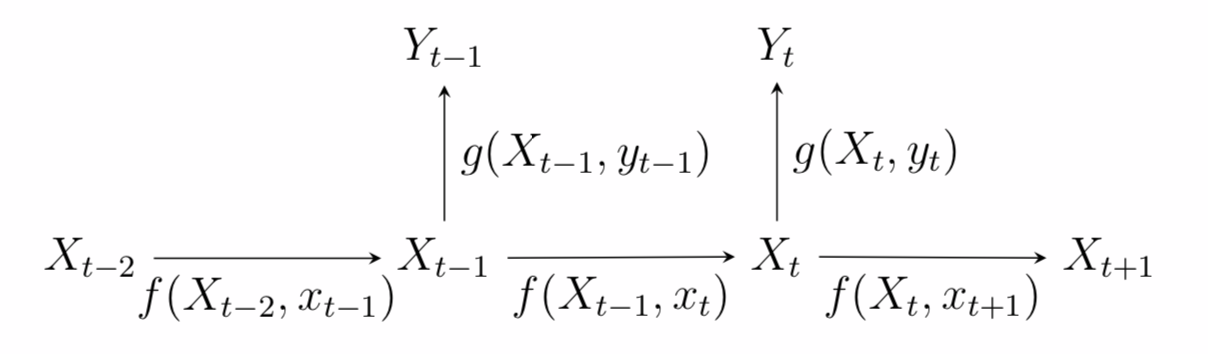
\includegraphics[width=0.6\textwidth]{figs/hmm_evol}
	\caption{Evolution of RVs in a HMM}
\end{figure}

\textbf{Note: }HMMs are significantly more `powerful' than state space models; there is no underlying assumption that evolution is linear. 

\ix{Joint Density}The joint density of $(X_0, Y_0, \ldots, X_k, Y_k)$ can be written straightforwardly:
\begin{align}
p(x_0, y_0, \ldots, x_k, y_k) &= \prod_{i=0}^k p(y_i| x_{i}, x_0, \ldots x_{i-1}, y_0, \ldots y_{i-1}) p(x_{i}| x_0, \ldots x_{i-1}, y_0, \ldots y_{i-1}) \nonumber \\&= p(x_0) g(x_k, y_k) \prod_{i=0}^k g(x_i, y_i) f(x_i, x_{i+1})
\end{align}
Examples of HMM models include:
\begin{enumerate}
	\item\ix{Gaussian State Space Model}In the Gaussian state-space model, the driving noises are Gaussian:
	\begin{align}
	X_{k+1} = aX_k + bW_{k+1} \hspace{1cm} Y_k = cX_k + dV_k
	\end{align}
	for $k=0, 1, \ldots$ where $V_k \sim \altmathcal{N}(0, 1)$, $W_k \sim \altmathcal{N}(0, 1)$ and $X_0 \sim \altmathcal{N}(\bar{\mu}_0, \bar{\sigma}_0)$ 
	
	\item\ix{Stochastic Volatility Model} The stochastic volatility model is:
	\begin{align}
	X_{k+1} = aX_{k-1} + bW_k \hspace{1cm} Y_k = c\exp \frac{X_k}{2} V_k
	\end{align}
	for $k=0, 1, \ldots$ where $V_k \sim \altmathcal{N}(0, 1)$, $W_k \sim \altmathcal{N}(0, 1)$ and $X_0 \sim \altmathcal{N}(\bar{\mu}_0, \bar{\sigma}_0)$ 
	
	\item A discrete valued Markov change, observed in Gaussian noise. $X_k \in S = \lbrace 1, \ldots, n \rbrace$ with:
	\begin{align}
	P(X_k = i_k | X_{k-1} = i_{k-1}) = P_{i_{k-1}, i_k}
	\end{align}
	$\vect{P}$ is the transition probability matrix with the sum of each row being $1$ (for correct normalisation). Given $X_k = i_k$, the observed process is:
	\begin{align}
		Y_k = c_{i_k} + d_{i_k} V_k
	\end{align}
	for $k=0, 1, \ldots$ where $V_k \sim \altmathcal{N}(0, 1)$. $c_1, d_1, \ldots, c_n, d_n$ are real valued constants. 
\end{enumerate}
\ix{Inference Objectives for HMMs}There are multiple possible inference objectives for the HMM model:
\begin{enumerate}
	\item \textbf{Filtering:} compute the density of the current hidden state. 
	\begin{align}
	p(x_k | y_0, \ldots, y_k)
	\end{align}
	
	\item \textbf{Prediction: } compute the future hidden state. 
	\begin{align}
	p(x_{k+m} | y_0, \ldots, y_k)
	\end{align}
	
	\item \textbf{Smoothing: } improve estimates of previous hidden states.
	\begin{align}
	p(x_{k-m} | y_0, \ldots, y_k)
	\end{align}
\end{enumerate}
HMMs have exact solutions for discrete values of $X_k$ and for continuous valued $X_k$ if the Gaussian state-space model is used. 

\qx{Exact Computations for the Discrete HMM}For the discrete valued HMM, the exact sequential computations are: 
\begin{align}
p(i_{k+1} | y_{0:k}) &= [\pi_k^T P]_{i_{k+1}} \\ 
\pi_{k+1}^T &= \frac{\pi_k^T P B_{k+1}}{\pi_k^T P B_{k+1} \vect{1}}
\end{align}
where $pi_k$ is the column vector of $p(x_k = i_k| y_{0:k})$, $\vect{1}$ is a column vector of ones and $B_k$ is defined as 
\begin{align}
B_k = \begin{bmatrix}
g(1, y_k) & & \\
& \ddots & \\
& & g(n, y_k)
\end{bmatrix}
\end{align}
\ix{Bayesian Kalman Filter Update Equations}In general, assuming that $p(x_k|y_{0:k})$ is known, the Kalman filter equations are:\qx{Derive this}
\begin{align}
p(x_{k+1}|y_{0:k}) &= \int p(x_k | y_{0:k}) f(x_k, x_{k+1})\ dx_k \\
p(x_{k+1}|y_{0:k+1}) &= \frac{p(x_{k+1}|y_{0:k}) g(x_{k+1}, y_{k+1})}{\int p(x_{k+1}|y_{0:k}) g(x_{k+1}, y_{k+1}) dx_{k+1}}
\end{align}

\qx{Bayesian Kalman Filter - Prove the Update Equations}For the special case of the Gaussian state space model, the Kalman filter prediction equation, assuming that $p(x_k| y_{0:k}) = \altmathcal{N}(\mu_k, \sigma_k)$, is
\begin{align}
\bar{\mu}_{k+1} = a\mu_k \hspace{1cm} \bar{\sigma}_{k+1} = a^2 \sigma_k + b^2
\end{align}
The update equations are then:
\begin{align}
\mu_{k+1} &= \bar{\mu}_{k+1}  + \frac{c\bar{\mu}_{k+1} }{c^2 \bar{\mu}_{k+1}  + d} (y_{k+1} - c \bar{\mu}_{k+1} ) \\
 \sigma_{k+1} &= \bar{\sigma}_{k+1} - \frac{c^2 \bar{\sigma}^2_{k+1}}{c^2 \bar{\sigma}^2_{k+1} + d^2}
\end{align}
Thus with an initial density for the first hidden state, the \emph{Bayesian Kalman Filter} equations are very straightforward to implement. 

\section{Importance Sampling}
Let $\pi(x)$ be a probability density function with $x \in \mathbb{R}^n$. Often, we want to compute integrals with respect to $\pi$:
\begin{align}
\expt{h(X)}{\pi} = \int h(x) \pi(x)\ dx
\end{align}
for some function $h: \mathbb{R}^n \rightarrow \mathbb{R}$.\ix{When do we use importance sampling?} In general, \textbf{it may not be possible to sample from $\pi$}, meaning that a direct Monte Carlo estimate cannot be computed. 

\ix{Importance Sampling}\emph{Important Sampling} estimates $\expt{h(X)}{\pi}$ using \emph{Monte Carlo} using some probability density function, $q(x)$, from which we can sample. 
\begin{align}
\expt{h(X)}{\pi} \simeq \frac{1}{N} \sum_{i=1}^N h(X^{(i)}) \underbrace{\frac{\pi(X^{(i)})}{q(X^{(i)})}}_{w^{(i)}} \hspace{0.25cm}\text{ where } X^{(i)} \stackrel{iid}{\sim} q
\end{align}
Note that this is an unbiased estimate.\qx{Show Unbiased} $w^{(i)}$ is the importance weight. 

\ix{Self-Normalised Importance Sampling}In general, it cannot be assumed that the target density normalises, as often it is difficult to calculate the correct normalising constant. Let $\pi(x) \geq 0\ \forall x$. Then, the \emph{Self Normalised Importance Sampling} estimate is constructed as follows:
\begin{align}
\expt{h(X)}{\pi^*} \simeq \frac{\sum_{i=1}^N h(X^{(i)}) w^{(i)}}{\sum_{i=1}^N w^{(i)}} \hspace{0.25cm}\text{ where } X^{(i)} \stackrel{iid}{\sim} q
\end{align}
\qx{Show Estimate \& Bias}Note that the denominator uses importance sampling (with the same set of samples) to estimate the normalising constant. Note that this estimate is biased. 

\ix{Central Limit}Let $X_1, \ldots$ be a sequence of iid RVs with $\expt{X_i}{} = 0$ and $\expt{X_i^2}{} = \sigma^2$. Define:
\begin{align}
Z_N = \frac{1}{\sqrt{N}} \sum_{i=1}^N X^{(i)}
\end{align}
As $N\rightarrow \infty$, the distribution of $Z_n$ approaches $\altmathcal{N}(0, \sigma^2)$. 

\qx{Efficiency Loss - Proof}Other that $q$, note that superscript $*$ denotes a normalised density, or quantities produced using normalised densities. Define
\begin{align}
S_1 &= \frac{1}{N} \sum_{i=1}^N h(X^{(i)}) w^*(X^{(i)}) \\
S_2 &= \frac{1}{N} \sum_{i=1}^N w^*(X^{(i)})
\end{align}
and note that the self-normalised importance sampling estimate can be expressed as $S_1 / S_2$. Additionally:
\begin{align}
s_1 = \expt{S_1}{} = \expt{h(X)}{\pi*} \hspace{1cm} s_2 = \expt{S_2}{} = 1
\end{align}
Now consider the variation of the sample about the target value:
\begin{align}
\frac{S_1}{S_2} - s_1 &= \frac{1}{S_2} (S_1 - S_2 s_1) \nonumber\\
&= \frac{1}{S_2} \frac{1}{N} \sum_{i=1}^N (h(X^{(i)}) - s_1) w^*(X^{(i)})
\end{align}
Note that each term in the summation has zero mean\qx{Show Zero Mean} and variance:\begin{align}
\sigma^2 &= \expt{(h(X) - s_1)^2 w^*(X)^2}{q} \nonumber \\
&= \expt{(h(X) - s_1)^2 w^*(X)}{\pi^*}
\end{align}
Applying the central limit theorem, for large $N$,
\begin{align}
\frac{S_1}{S_2} - s_1 \rightarrow \frac{1}{S_2} \frac{1}{\sqrt{N}} \altmathcal{N}(0, \sigma^2)
\end{align}
Also note that for large $N$, $S_2 \rightarrow 1$, meaning the the importance sampling estimate has the following asymptotic distribution:
\begin{align}
\frac{S_1}{S_2} \overset{\text{large }N}{\sim} \altmathcal{N}(\expt{h(X)}{\pi*}, \frac{\sigma^2}{N})
\end{align}
so the self-normalised importance sampling estimate is asymptotically unbiased. 

\ix{Typical Monte Carlo Variance} The variance of a Monte Carlo estimate, assuming sampling from the correct distribution could be performed, is:
\begin{align}
\frac{1}{N} \underbrace{\expt{(h(X) - \expt{h(X)}{\pi*})^2}{\pi^*}}_{\sigma_0^2}
\end{align}

Equating the variance of a normal Monte Carlo estimate and the self-normalised importance sampling estimate gives:
\begin{align}
N_{\text{IS}} = N \frac{\sigma^2}{\sigma_0^2}
\end{align}
Often $\sigma^2 / \sigma_0^2 > 1$, meaning that more samples from $q$ are required to match the quality of the estimate using $\pi^*$. There is a loss of efficiency due to the trial probability density function $q$ and the target. It can be difficult to find a good candidate for the trial distribution, especially as the dimension of the problem increases (the ratio between the variances can increase with the problem size). 

\section{Sampling Techniques for HMMs}
The\ix{Target Density} target density is the conditional density of all the states given all the observations.
\begin{align}
\pi_n^*(x_0, \ldots, x_n) = p(x_0, \ldots, x_n | y_0, \ldots, y_n) \propto \underbrace{p(x_0, y_0, \ldots, x_n, y_n)}_{\pi_n(x_0, \ldots, x_n)}
\end{align}
\ix{Trial Density}The trial distribution has the following Markov structure:
\begin{align}
q_n(x_0, \ldots, x_n) = q_0(x_0)q_1(x_0, x_1)\ldots q_n(x_{n-1}, x_n)
\end{align}
where each $q_i(x_{i-1}, x_i)$ is normalised in the second argument. Typically we may sample from the state transition density, $f(\cdot, \cdot)$. \ix{Importance Weights}Given this structure, the importance weights can be written:
\begin{align}
w(X_{0:n}^{(i)}) = \frac{p(X^{(i)}_0) g(X^{(i)}_0, y_0)}{q(X^{(i)}_0)} \frac{f(X^{(i)}_0, X^{(i)}_1) g(X^{(i)}_1, y_1)}{q(X^{(i)}_0, X^{(i)}_1)} \cdots \frac{f(X^{(i)}_{n-1}, X^{(i)}_n) g(X^{(i)}_n, y_n)}{q(X^{(i)}_{n-1}, X^{(i)}_n)} \label{eq:hmm_sample_pi}
\end{align}
\subsection{Sequential Importance Sampling}
The idea behind sequential importance sampling is to exploit the Markov structure of $q_n$ when sampling from it. Given samples, $X_{0:n}^{(i)} \sim q_n$, and weights, $w(X_{0:n}^{(i)})$, sequential importance sampling can be performed as follows:
\begin{enumerate}
	\item \ix{Extension}Sample $X_{n+1}^{(i)}$ from $q_{n+1}(X_{n}^{(i)}, x_{n+1})$ for each sample, $i$. Then, simply append the new sample onto the existing samples, $X_{0:n+1}^{(i)} = \begin{bmatrix}
	X_{0:n}^{(i)}, X_{n+1}^{(i)}
	\end{bmatrix}$.
	
	\item \ix{Weight Update}Re-weight each sample:
	\begin{align}
	w_{n+1}^{(i)} = w_{n+1}^{(i)} \underbrace{\frac{f(X^{(i)}_{n}, X^{(i)}_{n+1}) g(X^{(i)}_{n+1}, y_n)}{q(X^{(i)}_{n}, X^{(i)}_{n+1})}}_{u_{n+1}^{(i)}}
 	\end{align}
 	$u_{n+1}^{(i)}$ is known as the incremental weight. This expression for the incremental weight follows directly from Eq. \ref{eq:hmm_sample_pi}.
\end{enumerate}

\ix{Problem with Sequential Importance Sampling}The problem is sequential importance sampling is that eventually the weights will collapse, with most of the weights becoming small and one larger than the rest. Thus, one of the $N$ normalised weights ($w^{(i)}_n / \sum_j w^{(j)}_n$) will be close to $1$, meaning that the self-normalised estimate will collapse to a single sample estimate.

\ix{Developing a Solution}We note that samples with small normalised weights should not be carried forward, whilst those with larger normalised weights should. Additionally, the population size should be kept at the original level, $N$, or only a single sample will remain. Resampling is one technique of resolving this problem. 

\subsection{Resampling}\begin{algorithm}[H]
	\DontPrintSemicolon
	\SetKwInOut{Input}{Input}
	\Input{$N$ weighted samples, ($X_{0:n}^{(i)}, w_n^{(i)}$) which unbiasedly approximate $\pi_n$ i.e. \begin{align}
		\expt{h_n(X_{0:n}^{(i)}) w_n^{(i)}}{} =\int h_n(x_{0:n}) \pi_n(x_{0:n})\ dx_{0:n}
		\end{align}}\;
	Let $W_n = \sum_j w_n^{(j)}$ \;
	
	\For{$i = 1, \ldots, N$}{
		Sample $J$ from the set $\lbrace 1,\ldots, N \rbrace$ with $Pr(J = j) = w_n^{(j)}/W_n$\;
		
		$X_{0:n}^{(i)} \leftarrow X_{0:n}^{(J)}$\;
		
		$w_{n}^{(i)} \leftarrow W_n / N$\;
	} \;
	\caption{Resampling}
\end{algorithm}

\qx{Proof: Unbiasedness of Resampling}The unbiased of resampling is easy to show, given that the input samples are also biased. To complete this proof, simply write down and rearrange the expected value of the output, considering first the randomness in $J$. 

\subsection{Sequential Importance Sampling with Resampling}
The resampling technique is developed as follows: after resampling and reweighting occurs, the particle is then extended and weighted according to the sample generated i.e. 
\begin{align}
X_{n+1}^{(i)} &\sim q_{n+1}(X_{0:n}^{(i)}, x_{n+1}) \\
w_{n+1}^{(i)} &= \underbrace{\frac{W_n}{N}}_{w_n^{(i)}} \underbrace{\frac{f(X^{(i)}_{n}, X^{(i)}_{n+1}) g(X^{(i)}_{n+1}, y_n)}{q(X^{(i)}_{n}, X^{(i)}_{n+1})}}_{u_{n+1}^{(i)}}
\end{align}
This gives an unbiased estimate of $\pi_{n+1}$\qx{Verify Unbiasedness} that can be verified by considering:
\begin{align}
\expt{h_{n+1}(X_{0:n}^{(J)}, X_{n+1}^{(i)}) w_{n+1}^{(i)}}{}
\end{align}
When evaluating this, the randomness in each original sample, the value of $J$, and the value of $X_{n+1}^{(i)}$ must be considered in reverse order. 

\textbf{The Particle Filter} is this technique, applied specifically to Hidden Markov Models. Note that by setting $h_T(x_{0:T}) = 1$, the particle filter calculates the probability of the observed data. 

\subsection{Analysis of the Particle Filter}
\ix{Pertinent Questions}When using the particle filter, we want to know:
\begin{enumerate}
	\item Do the number of particles, $N$, need to increase with the length of the time-series to get a stable estimate of $p(y_{0:T})$? 
	\item How does the particle filter compare to normal sequential importance sampling without the re-sampling steps?
\end{enumerate}

Consider the average sum of weights at time $T$:\qx{Prove this Expansion}
\begin{align}
p(y_{0:T}) &\simeq \frac{W_T}{N} \nonumber  \\
&= \frac{W_{T-1}}{N} \sum_{i=1}^N \frac{u_T^{(i)}}{N}  \nonumber \\
&= \Big( \frac{1}{N} \sum_{i=1}^N \frac{p(X_0^{(i)})g(X_0^{(i)})}{q_0(X_0^{(i)})}\Big) \prod_{j=1}^T \Big( \sum_{i=1}^N \frac{u_j^{(i)}}{N} \Big)
\end{align}
\ix{Simplifying Example}This is not easy to analyse in general. Thus, let the hidden state process be IID according to $p(\cdot)$. Then:
\begin{align}
p(y_{0:T}) = \prod_{i=0}^Tp(y_i)
\end{align}
with $p(y_i) = \int p(x_n)g(x_n, y_n) dx_n$. Additionally, consider $q_n(x_{n-1}, x_n) = p(x_n)$. Then:
\begin{align}
p(y_{0:T}) \simeq \prod_{j=0}^T \Big( \sum_{i=1}^N \frac{g(X_j^{(i)}, y_j) }{N} \Big) = \prod_{j=0}^T \frac{U_j}{N}
\end{align}
Consider the variance of this estimate, noting independence:
\begin{align}
\frac{\text{var}\ [\frac{W_T}{N}]}{p(y_0)^2 \cdots p(y_T)^2 } = \mathbb{E} \Bigg\lbrace \Bigg( \frac{U_0}{Np(y_0)} \Bigg)^2 \Bigg\rbrace \cdots \mathbb{E} \Bigg\lbrace \Bigg( \frac{U_T}{Np(y_T)} \Bigg)^2 \Bigg\rbrace - 1
\end{align}
For any value of $n$:\qx{Show This}
\begin{align}
\mathbb{E} \Bigg\lbrace \Bigg( \frac{U_n}{Np(y_n)} \Bigg)^2 \Bigg\rbrace = 1 + \frac{1}{N} \underbrace{\text{var}\ \Bigg[\frac{g(X_n, y_n)}{p(y_n)} \Bigg]}_{c_n}
\end{align}
Therefore, noting that $1 + \frac{c_n}{N} < \exp(\frac{c_0}{N})$ by Taylor expansion, we note that:
\begin{align}
\frac{\text{var}\ [\frac{W_T}{N}]}{p(y_0)^2 \cdots p(y_T)^2 } < \exp \Big( \frac{c_0 + \cdots + c_T}{N} \Big) - 1
\end{align}
Giving a variance which grows with $T$, unless $N$ is also increased with $T$.

\section{Model Calibration} 
\ix{Parametrising a HMM}A hidden Markov model can be parametrised by a vector by modifying the state transition density and observation density to depend on a parameter, $\theta \in \mathbb{R}^d$ i.e. 
\begin{align*}
f_\theta(x_{k-1}, x_k) \hspace{1cm} g_\theta(x_k, y_k)
\end{align*}
\ix{Choosing $\theta_k^*$}A typical approach used to choose these parameters is to use the \emph{maximum likelihood principle}:
\begin{align}
\theta_k^*  = \arg \max_\theta \underbrace{\log p_{\theta}(y_{0:k})}_{\altmathcal{L}_k(\theta)}
\end{align}
which, under some assumptions, provides a consistent estimator i.e. $\theta_k^* \rightarrow \theta^*$ as the data length increases and $\theta^*$ is the `optimal' value. \ix{Why is this hard?}However, we do not observe the hidden states and thus it is difficult to find the maximiser. We resort to iterative methods.

\subsection{Gradient Methods}
One simple approach is to apply gradient ascent:
\begin{align}
\theta^{(i+1)} = \theta^{(i)} + \eta_i \nabla_\theta \altmathcal{L}(\theta^{(i)})
\end{align} 
where $\nabla_\theta$ denotes the vector gradient in the usual way and $\lbrace \eta_i \rbrace$ is a positive step size sequence tending to zero. The parameter will converge to a local maximum of the likelihood, which may not necessarily be the global maximiser. Typically, we may use \emph{Stochastic Approximation} \ix{Stochastic Approximation} where a Monte Carlo estimate of the gradient is used, in which case the step size sequence should be chosen such that the step sizes are positive, tend to zero but with $\sum_i \eta_i = \infty$. A typical choice is:
\begin{align}
\eta_i = \frac{1}{i^\alpha}
\end{align}
with $\alpha \in [0.5, 1]$. Fixed step sizes give oscillatory behaviour around a maximum. 

It can be shown that:\qx{Stochastic Optimisation}
\begin{align}
\frac{\partial \altmathcal{L}(\theta)}{\partial \theta_k} = \int \Bigg( \frac{\partial}{\partial \theta_k} \log p_\theta(x_{0:n}, y_{0:n})\Bigg) p_\theta(x_{0:n}| y_{0:n})\ dx_{0:n}
\end{align}
which can be calculated using the particle filter. Additionally, it is easy to show that\qx{Proof}:
\begin{align}
\frac{\partial}{\partial \theta_k} \log p_\theta(x_{0:n}, y_{0:n}) = \sum_{j=1}^n \Bigg( \frac{\partial}{\partial \theta_k} \log f_\theta(x_{j-1}, x_j) + \frac{\partial}{\partial \theta_k} \log g_\theta(x_j, y_j) \Bigg)
\end{align}

\subsection{Expectation Maximisation}
The EM algorithm is an alternative iterative procedure for maximising the log-likelihood. Define\ix{Auxiliary Function}:
\begin{align}
\altmathcal{Q}(\theta, \theta') = \int \log \lbrace p_{\theta'}(x_{0:k}, y_{0:k})  \rbrace p_\theta(x_{0:k}| y_{0:k}) dx_{0:k}
\end{align}
$\theta$ is the current best guest of the global maximiser and we optimise over $\theta'$. 
\qx{Prove using Jensen}Considering the strictly concave function $\log(x)$ and the variable $\frac{p_{\theta'}}{p_\theta}$, Jensen's Inequality directly implies that for any $\theta' \neq \theta$:
\begin{align}
\int \log p_{\theta'}(x_{0:k} | y_{0:k}) p_\theta(x_{0:k}|y_{0:k})\ dx < \int \log p_{\theta}(x_{0:k} | y_{0:k}) p_\theta(x_{0:k}|y_{0:k})\ dx
\end{align} 
which effectively states that the average log likelihood under the true density is larger than under any other density. \qx{Rearrange as required}Rearranging gives:
\begin{align}
\log p_{\theta'}(y_{0:k}) - \log p_{\theta}(y_{0:k}) > \altmathcal{Q}(\theta, \theta') - \altmathcal{Q}(\theta, \theta)
\end{align}
Thus by maximising over $\theta'$ are each step means that the log likelihood will increase. The EM algorithm repeatedly maximises the auxiliary function. The E-step computes $\altmathcal{Q}(\theta, \theta')$ and the M-step maximises this over $\theta'$. 

For the general HMM we cannot compute the integral defining $\altmathcal{Q}(\theta, \theta')$ though we can for the Gaussian state-space model. 

\subsubsection*{EM for Exponential Family Models}
\ix{Exponential Family}A HMM belongs to the exponential family if:
\begin{align}
f_\theta(x_{n-1}, x_n) g_\theta(x_n, y_n) = h(x_{n-1}, x_n, y_n) \exp \Big[ \phi(\theta)^T S(x_{n-1}, x_n, y_n) - m(\theta)\Big]
\end{align}
where $\phi(\theta)$ and $S(x_{n-1}, x_n, y_n)$ are vector valued functions of the same dimension. Then:
\begin{align}
p_{\theta'}(x_{0:k}, y_{0:k}) = \exp \Bigg[ \sum_{n=0}^k \phi(\theta')^T S(x_{n-1}, x_n, y_n) - (k+1) m(\theta') \Bigg] \times \prod_{n=1}^k h(x_{n-1}, x_n, y_n)
\end{align}
The\qx{Derive This} maximisation step then reduces to maximising:
\begin{align}
\phi(\theta')^T \underbrace{ \int \Bigg(\sum_{n=0}^k  S(x_{n-1}, x_n, y_n) \Bigg) p_\theta(x_{0:k}| y_{0:k})\ dx_{0:k}}_{\bar{S}} - (k+1) m(\theta')
\end{align}
$\bar{S}$ can be computed easily using the particle filter, and note that it is independent of $\theta'$. Then, we require:
\begin{align}
\max_\theta \phi(\theta)^T \bar{S} + (k+1)m(\theta') 
\end{align}
which can be solved easily, but note that the type of stationary point found needs to be checked. 

\ix{Linking Gradient Ascent and EM}Note that:
\begin{align}
\frac{\partial \altmathcal{L}(\theta)}{\partial \theta_k} = \frac{\partial \altmathcal{Q}(\theta, \theta')}{\partial \theta'}\Bigg|_{\theta' = \theta}
\end{align}
which can be seen easily simply via substitution. Gradient ascent replaces the maximisation step of the EM algorithm; the new value of $\theta'$ is the current value plus a small change in the direction of increasing the auxiliary function.  


\end{document}
